\chapter{Знакомство с  Lego Mindstorms NXT 2.0}
{\bfseries Анонс:}\\\\
Lego Mindstorms NXT 2.0. Практикум «Самый длинный мост». Практикум «Неведомый зверь». Терминология.\\\\
{\bfseries Цели:}
\begin{itemize}
	\item{}{\bfseries Обучающие:} Ознакомить учащихся с составляющими набора для создания роботов. Освоить  основные принципы соединения деталей. Обучить учащихся общепринятой терминологии.
	\item{}{\bfseries Воспитательные:} Познакомить учащихся друг с другом, снизить уровень их тревожности.\\
\end{itemize}	
{\bfseries Ход занятия:}\\\\
\begin{tabular}{lll}
	\hyperlink{lesson2x1}{1. Организационный момент} & Презентация & (5 мин)\\
	\hyperlink{lesson2x2}{2. Lego Mindstorms NXT 2.0} & Презентация & (30 мин) \\
	\hyperlink{lesson2x3}{3. «Самый длинный мост»} & Игра & (30 мин) \\
	\hyperlink{lesson2x4}{4. «Неведомое животное»} & Игра & (40 мин)\\
	\hyperlink{lesson2x5}{5. Основы терминологии} & Рефлексия & (5 мин)\\
\end{tabular}\\\\

{\hypertarget{lesson2x1}{\blackBlueText{I.Организационный момент}}}\\\\

Сегодня учащимся предстоит собрать свои первые конструкции и познакомиться с набором. Каждой паре предоставляется свое рабочее пространство, следует проследить, что бы оно было достаточно большим, что бы разместить на нем коробку с деталями и иметь площадку для творчества. Попросите убрать все посторонние предметы со столов, ничего кроме наборов в этот раз не понадобится.

Изначально раздайте учащимся только блоки, моторы и датчики. С одной стороны это позволит им в процессе знакомства с набором держать в руках предметы о которых идет речь, с другой не даст отвлечься на собирание чего-то своего из набора деталей. Набор с деталями следует раздать только в начале упражнения «Самый длинный мост».\\\\

{\hypertarget{lesson2x2}{\blackBlueText{II. Lego Mindstorms NXT 2.0}}}\\\\

Мы будем использовать набор Lego Mindstorms NXT 2.0 8547. В каждом наборе содержится 619 деталей, включая очень мелкие, поэтому, чтобы было легко их находить и хранить нужна четкая система. В качестве кейсов для хранения предлагается использовать следующие коробки для инструментов
\begin{figure}[h!]
	\begin{center}
		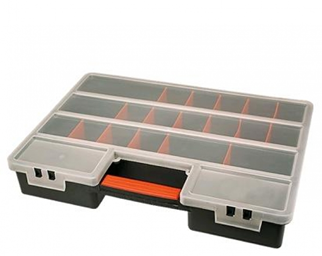
\includegraphics[width=1\linewidth]{chapters/chapter2/images/1}
		\caption{Ящик для хранения деталей.}
		\label{ris:image2x1}
	\end{center}
\end{figure}			

В таком случае удобной оказывается следующая раскладка деталей:
\begin{figure}[h!]
	\begin{center}
		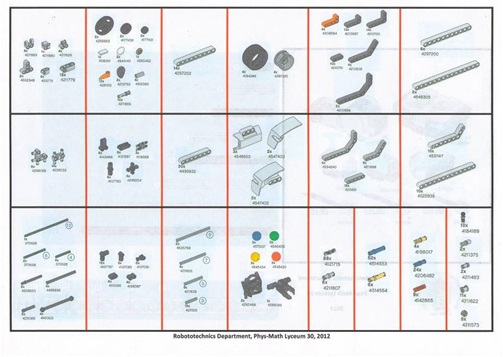
\includegraphics[width=1\linewidth]{chapters/chapter2/images/2}
		\caption{Раскладка деталей набора 8547 (\yellowText{Приложение}).}
		\label{ris:image2x2}
	\end{center}
\end{figure}		

При использовании образовательной версии набора 9797 LEGO MINDSTORMS Education NXT Base Set вкладыш для хранения деталей уже входит в набор.

С другой стороны раскладки удобно напечатать в масштабе 1:1 балки и оси, что бы при переборе наборов просто сравнивать детали с рисунком.
\clearpage
\begin{figure}[h!]
	\begin{center}
		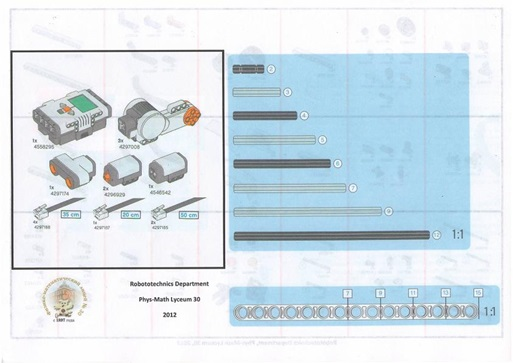
\includegraphics[width=1\linewidth]{chapters/chapter2/images/3}
		\caption{Оборотная сторона раскладки (\yellowText{Приложение}).}
		\label{ris:image2x3}
	\end{center}
\end{figure}		

Заламинированную раскладку деталей рекомендуется вложить в каждый набор. К набору имеет смысл приклеить кармашек, с вложенным листом учета деталей (Приложение).

В конце каждого занятия робот полностью разбирается, все детали раскладываются по местам, а набор сдается преподавателю под роспись. Это позволяет быстро освоить основные моменты конструирования, за счет частой сборки- разборки, а так же повысить ответственность учащихся и уменьшить естественную убыль деталей. Так же коробка с рис. показала себя как удобная в транспортировке при поездках на соревнования в другие города.\\\\	
Помимо деталей конструктора в стандартный набор входят:
\begin{itemize}
	\item Блок NXT. В неформальной литературе так же часто встречается названия брик (brick) и кирпич. На техническом языке  - это 32-битовый микроконтроллер ARM7 256 КБайт FLASH, 64 КБайт RAM  и 8-битовый микроконтроллер AVR 4 Кбайта FLASH, 512 байт RAM, а также беспроводный канал Bluetooth Class II V 2.0. А проще говоря~--- «мозг» нашего робота. К нему будут подключаться все сенсоры (глаза, уши, нос и т.п. робота) и он же будет давать команды моторам (рукам и ногам).
	\clearpage
	\begin{figure}[h!]
		\begin{center}
			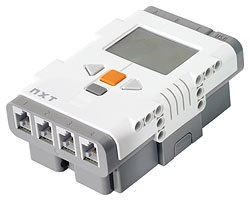
\includegraphics[width=0.65\linewidth]{chapters/chapter2/images/4}
			\caption{Блок NXT.}
			\label{ris:image2x4}
		\end{center}
	\end{figure}	
	
	Блок имеет 3 разъема для подключения моторов (A,B,C), 4 разъема для сенсоров (1,2,3,4) и разъем USB для соединения с компьютером. На передней панели расположен дисплей и 4 кнопки. С помощью оранжевой кнопки можно включить или выключить питание, светло-серые стрелки необходимы при перемещении влево - вправо по меню NXT, а темно-серая кнопка удаляет или возвращает пользователя в предыдущее меню.  На задней стороне блока находится отделение для аккумуляторов. Блок может работать от фирменного аккумулятора Lego, а так же обычных 6 батареек или аккумуляторов типа АА.
	\begin{figure}[h!]
		\begin{center}
			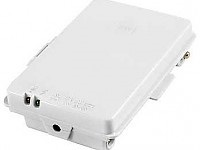
\includegraphics[width=0.65\linewidth]{chapters/chapter2/images/5}
			\caption{Аккумуляторный блок Lego.}
			\label{ris:image2x5}
		\end{center}
	\end{figure}
	
	Так же блок оснащен громкоговорителем, что позволяет проигрывать ему различные звуки при воспроизведении программы.		 
	\item Три сервопривода. Могут вращаться в любом направлении. Скоростью вращения моторов можно программно управлять. В приводы встроен счетчик числа оборотов, точнее градусов на которые повернулся привод.
	\begin{figure}[h!]
		\begin{center}
			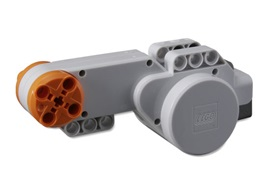
\includegraphics[width=0.6\linewidth]{chapters/chapter2/images/6}
			\caption{Сервопривод.}
			\label{ris:image2x6}
		\end{center}
	\end{figure}
	
	\item Ультразвуковой сенсор. (Особенно любим детьми, после выхода одноименного мультика имеет ласковую кличку Валли). Посылает ультразвуковую волну и принимает ее, отраженную от преграды. По времени прохождения и известной скорости волны определяет расстояние до преграды. Не работает с шероховатыми поверхностями, из-за слишком сильного рассеивания ими звуковых волн.
	\begin{figure}[h!]
		\begin{center}
			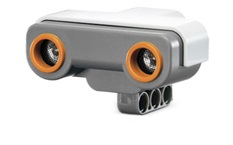
\includegraphics[width=0.6\linewidth]{chapters/chapter2/images/7}
			\caption{Ультразвуковой сенсор.}
			\label{ris:image2x7}
		\end{center}
	\end{figure}
	
	\item Сенсор касания. Просто кнопка. Возвращает состояние нажата/не нажата.
	\begin{figure}[h!]
		\begin{center}
			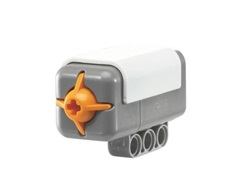
\includegraphics[width=0.6\linewidth]{chapters/chapter2/images/8}
			\caption{Сенсор касания.}
			\label{ris:image2x8}
		\end{center}
	\end{figure} 
	
	\item Сенсор освещенности. Входит в набор Education. Возвращает значение освещенности поверхности в условных единицах от 0 (черное) до 255 (белое).
	\begin{figure}[h!]
		\begin{center}
			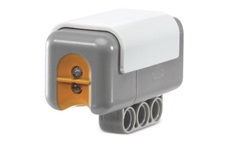
\includegraphics[width=0.6\linewidth]{chapters/chapter2/images/9}
			\caption{Сенсор освещенности.}
			\label{ris:image2x9}
		\end{center}
	\end{figure}
	
	\item Сенсор цвета. Может использоваться в одном из пяти режимов: Lego Color-Red, Lego Color-Green, Lego Color-Blue, Lego Color-RGB и Lego Color. В первых четырех работает как датчик освещенности, подсвечивая себе путь светодиодом соответствующего цвета (цветов). В последнем режиме датчик способен различать цвета.
	\begin{figure}[h!]
		\begin{center}
			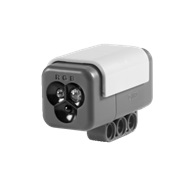
\includegraphics[width=0.6\linewidth]{chapters/chapter2/images/10}
			\caption{Сенсор цвета.}
			\label{ris:image2x10}
		\end{center}
	\end{figure}
\end{itemize}

{\hypertarget{lesson2x3}{\blackBlueText{III. «Самый прочный мост»}}}\\\\

Итак, набор продемонстрирован, правила раскладки деталей оговорены. Самое время для первого практического задания!

Учащиеся разбиваются на группы по 3--4 человека. У каждой группы в распоряжении 1 набор. Задача~--- построить самый прочный мост между двумя столами, находящимися на расстоянии 50 см. Самым прочным считается мост, выдержавший наибольший груз в течение 3 секунд.

{\slshape Возможны вариации на тему «самый длинный мост», «самая высокая башня» и т.д. Главное в этом задании - это возможность детям  после довольно долгого для них обзора, наконец, потрогать набор, попробовать разные варианты соединения деталей, познакомиться друг с другом.}\\\\

{\hypertarget{lesson2x4}{\blackBlueText{IV. «Неведомое животное»}}}\\\\

Учащиеся  разбиваются по парам. Одному человеку в паре предлагается собрать из деталей одного набора любое фантастическое животное за 10--15 минут. Второй участник не должен видеть ни процесса, ни результата (в это время можно предложить ему заполнить информационный лист из Приложения). Затем автору зверя предлагается объяснить своему товарищу, как собрать такого же~--- при этом напарники по-прежнему не видят друг друга и результаты своего труда.

Как правило, в этот момент, по всему классу раздаются диалоги следующего содержания:

- А теперь берешь вот ту серую штучку с пимпочкой и двумя усиками, засовываешь в нее синий треснутый цилиндрик \dots 

-Тот который с колечком или со вштыркой?\\
Возможные результаты подобного творчества представлены на \greenText{рис}.\\\\
\greenText{Рис.}\\\\

Затем следует провести игру еще раз, поменяв напарников ролями.\\\\

{\hypertarget{lesson2x5}{\blackBlueText{V. Основы терминологии}}}\\\\

В конце задания, вместе с учащимися следует проанализировать основную проблему с которой они столкнулись: проблема коммуникации. Для успешной работы в дальнейшем надо договориться о единых названиях для всех деталей. Можно обсудить, что в принципе, названия могут быть любыми, но если мы хотим  в дальнейшем общаться и с другими людьми, стоит выбрать общепринятые названия.

Раздаточный материал: Названия деталей (\yellowText{Приложение}).

Названия стоит проговорить вслух и посоветовать носить с собой раздатку в качестве шпаргалки, пока названия не запомнятся. Впредь использование самостоятельной терминологии рекомендуется аккуратно пресекать.